\section{From Microscopic to Mesoscopic Descriptions}

We have previously established that starting from the complete electron-phonon Hamiltonian and applying the weak-coupling approximation allows us to systematically integrate out the phononic degrees of freedom. This procedure yields an effective Hamiltonian governed purely by an attractive electron-electron interaction, \( V_{e^--e^-} \propto -|g_{\text{eff}}|^2 \). By analyzing this restricted two-body problem within a narrow momentum annulus surrounding the Fermi surface, we demonstrated that this effective attraction supports a stable bound state (\( E_2 < 0 \)). This is a profoundly non-trivial theoretical consequence, given the strong inherent Coulomb repulsion between bare electrons in a vacuum.

\begin{remark}
    This intellectual paradigm of integrating out collective bosonic modes to generate effective interactions between fundamental fermions is not exclusive to condensed matter physics. An elegant analogy exists in the realm of Cavity Quantum Electrodynamics (Cavity QED), a field significantly advanced by Serge Haroche (awarded the 2012 Nobel Prize in Physics). In both disciplines, the core physical phenomena emerge from the intricate interplay between microscopic elements (such as electrons mapping to micro degrees of freedom) and collective bosonic modes (such as phonons or cavity photons mapping to collective degrees of freedom).
\end{remark}

Moving forward, our current objective is to formally bridge the microscopic and mesoscopic descriptions of these interacting gases. At the two-body level, we will employ the quantum \textbf{T-matrix} to connect microscopic parameters (specifically the universal atomic interaction defined by the scattering length \( a \)) to the macroscopic properties of the effective interaction potential. Subsequently, we will tackle the full many-body grand-canonical problem by deploying Mean-Field approximations and the Bogoliubov transformation, methodologies mathematically homologous to those utilized for studying weakly interacting Bose gases.

\subsection{The Effective Attractive Potential}

To capture the essential physics of the Fröhlich mechanism, specifically the crucial detail that the phonon-mediated attraction only overcomes Coulomb repulsion for electrons energetically adjacent to the Fermi surface, the effective attractive potential is explicitly modeled by a piecewise function:
\begin{equation} \label{eq:bcs_potential}
    V(\mathbf{k}', \mathbf{k}) = \begin{cases}
        -g_{\text{e,ph}}^2 & \text{if } |\epsilon_k - \mu| < \hbar\omega_D \text{ and } |\epsilon_{k'} - \mu| < \hbar\omega_D, \\
        0                  & \text{elsewhere,}
    \end{cases}
\end{equation}
where \( g_{\text{e,ph}} \) represents the effective coupling constant between the electrons and phonons, \( \mu \) is the chemical potential of the electron gas (recalling that in the low-temperature limit \( T \to 0 \), the chemical potential intimately approaches the Fermi energy, \( \mu(T) \xrightarrow{T \to 0} E_F \)), \( \epsilon_k \) is the non-interacting kinetic energy of the fermion, and \( \omega_D \) is the characteristic Debye frequency of the ionic lattice.

By analyzing the explicit energy bounds in the expression for the potential \eqref{eq:bcs_potential}, we clearly see a profound physical restriction: only those electrons located within a remarkably narrow energy shell surrounding the Fermi sphere are permitted to interact attractively with each other.

\begin{figure}[H]
    \begin{minipage}{0.5\textwidth}
        \centering
        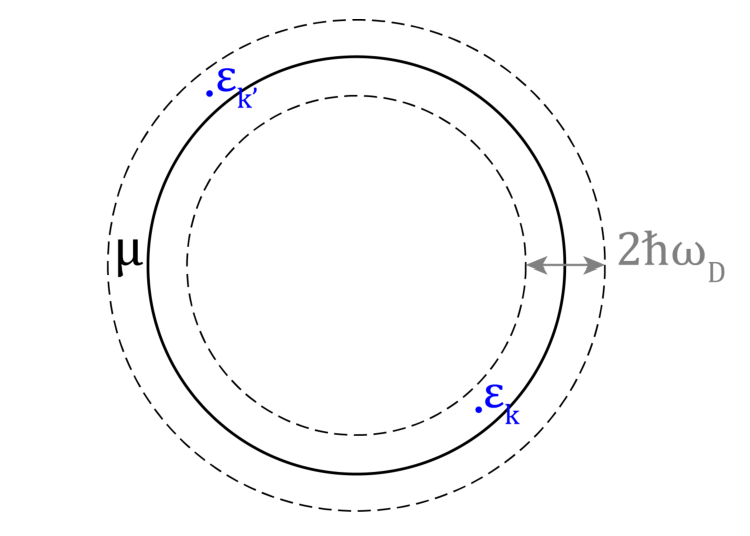
\includegraphics[width=0.8\textwidth]{img/2-bcs_energy_shell.png}
    \end{minipage}
    \hfill
    \begin{minipage}{0.45\textwidth}
        \caption{The model of the potential $V(\mathbf{k}', \mathbf{k})$ for superconductors is given by \eqref{eq:bcs_potential} and it involves just the fermions with energies $\epsilon_k$ and $\epsilon_{k'}$ residing strictly within a tiny energy shell of width $2\hbar\omega_D$ centered around the Fermi energy.}
        \label{fig:bcs_energy_shell}
    \end{minipage}
\end{figure}

To express this restricted interaction more compactly, it is highly advantageous to introduce a dimensionless cut-off function \( w_k = \Theta(\hbar\omega_D - |\epsilon_k - \mu|) \), where \( \Theta \) denotes the standard Heaviside step function. Utilizing this notation, the piecewise potential \eqref{eq:bcs_potential} can be elegantly rewritten in a strictly factorized form:
\begin{equation} \label{eq:bcs_potential_separable}
    V(\mathbf{k}', \mathbf{k}) = -g_{\text{e,ph}}^2 w_k w_{k'}.
\end{equation}
This mathematically represents the localized attractive potential acting exclusively between fermions scattered around the Fermi energy in a superconductor. Note that this specific theoretical form of the potential is entirely \emph{separable}; the dependence on the incoming momentum \( \mathbf{k} \) and the outgoing momentum \( \mathbf{k}' \) factors into independent terms, a property that will dramatically simplify the subsequent many-body calculations.

The theoretical framework developed here for electrons in solid-state crystal lattices can also be seamlessly applied to model ultracold Fermi gases. In these synthetic quantum systems, the microscopic interactions between two distinct particles occurring at different momenta are analogously modeled using a separable potential:
\[
    V_{\mathbf{k}',\mathbf{k}} = v_0 w_{\mathbf{k}} w_{\mathbf{k}'}.
\]
This structure is mathematically identical to the effective electron-electron potential derived previously. However, for ultracold atomic Fermi gases, the interaction is dictated directly by nature, and the fundamental physical parameter used to describe it is the scattering length \( a \). Typically, for these highly tunable atomic interactions, this characteristic value is on the order of \( a \simeq 100 a_0 \), where \( a_0 \) represents the Bohr radius.

\subsection{Ultracold Fermi Gases}

As previously established, the macroscopic theoretical framework developed for BCS superconductivity can be seamlessly adapted to study synthetic quantum systems of ultracold Fermi atoms. In these highly controlled atomic systems, the effective interparticle interaction possesses a very short range compared to the average interparticle distance. Because of this extreme separation of scales, it is highly convenient to model the interaction using a separable potential in momentum space:
\[
    V(\mathbf{k}', \mathbf{k}) = v_0 w_k w_{k'},
\]
where \( w_k = \Theta(k_0 - k) \) utilizes the Heaviside step function to introduce a strict ultraviolet momentum cutoff \( k_0 \), and \( v_0 \) represents the bare interaction strength. Formally, this separable potential is structurally homologous to the one utilized for modeling effective electron-phonon interactions in conventional superconductors.

\subsubsection{Definition of Scattering Length and the T-Matrix}

For a genuinely short-range contact potential in position space, the corresponding cutoff in momentum space must theoretically be taken to infinity, meaning \( k_0 \to \infty \). We thus need to understand how to appropriately treat this divergent limit mathematically. The core physical principle is that as the cutoff \( k_0 \) goes to infinity, the bare interaction parameter \( v_0 \) must simultaneously change (renormalize) with \( k_0 \) in a precise manner in order to keep the physically observable, macroscopic scattering length \( a \) strictly constant.

To rigorously connect the mesoscopic properties of the effective potential to the universal microscopic property given by the scattering length, we introduce the \textbf{T-matrix}, denoted as \( T(\mathbf{k}', \mathbf{k}, z) \), where \( z \in \mathbb{C} \) is a complex energy parameter. This T-matrix satisfies the fundamental Lippmann-Schwinger integral equation:
\[
    T(\mathbf{k}', \mathbf{k}, z) = V(\mathbf{k}', \mathbf{k}) + \int \frac{d^3 k''}{(2\pi)^3} \frac{V(\mathbf{k}', \mathbf{k}'')}{z - \frac{(k'')^2}{2m_r}} T(\mathbf{k}'', \mathbf{k}, z),
\]
where \( m_r \) is the reduced mass of the colliding two-body system. For a gas of identical fermions of mass \( m \), the reduced mass is simply \( m_r = m/2 \).

The formal relationship linking the T-matrix to the physical scattering length \( a \) is established by evaluating the T-matrix at zero incoming and outgoing momenta, and precisely at zero energy (\( z = 0 \)):
\begin{equation} \label{eq:scattering_length_definition}
    T(\mathbf{0}, \mathbf{0}, 0) = \frac{2\pi\hbar^2}{m_r} a.
\end{equation}
By invoking this definition, we are directly translating the physical requirement of a fixed scattering length \( a \) into a precise mathematical condition on the bare interaction strength \( v_0 \) as a function of the ultraviolet cutoff \( k_0 \). This equation elegantly bridges the two scales: \( T(\mathbf{0}, \mathbf{0}, 0) \) encapsulates the mesoscopic properties depending on the specific potential approximations, while \( a \) represents the universal microscopic property of the atoms. Furthermore, the scattering length \( a \) is directly related to the standard physical scattering amplitude function \( f(\mathbf{k}', \mathbf{k}) \) evaluated at zero momentum:
\[
    a = -f(\mathbf{0}, \mathbf{0}) = \frac{m_r}{2\pi\hbar^2} T(\mathbf{0}, \mathbf{0}, 0).
\]

\subsubsection{Renormalization of the Bare Coupling Strength}

We now wish to solve the integral differential equation for the T-matrix using our specific separable potential \( V(\mathbf{k}, \mathbf{k}') = v_0 w_k w_{k'} \). Substituting this into the Lippmann-Schwinger equation yields:
\[
    T(\mathbf{k}, \mathbf{k}', z) = v_0 w_{\mathbf{k}} w_{\mathbf{k}'} + \int \frac{d^3 k''}{(2\pi)^3} \frac{v_0 w_{\mathbf{k}} w_{\mathbf{k}''}}{z - \frac{(k'')^2}{2m_r}} T(\mathbf{k}'', \mathbf{k}', z).
\]

To proceed, we make a highly reasonable physical ansatz for the functional form of the T-matrix. Since the potential is non-zero exclusively when the momenta reside inside the energy shell (the momentum annulus), it is mathematically sound to assume that the T-matrix shares this exact property, effectively separating the momentum dependence from the complex energy parameter \( z \):
\[
    T(\mathbf{k}, \mathbf{k}', z) = w_{\mathbf{k}} w_{\mathbf{k}'} T(z).
\]
Let us rigorously verify why this factorization is justified:
\begin{itemize}
    \item If the outgoing momentum \( \mathbf{k}' \) is \textbf{outside} the annulus, the cutoff function vanishes by definition (\( w_{\mathbf{k}'} = 0 \)). Consequently, both the bare potential term and the integral term vanish identically, trivially yielding \( T = 0 \).
    \item If the incoming momentum \( \mathbf{k} \) is \textbf{outside} the annulus, the first term \( v_0 w_{\mathbf{k}} w_{\mathbf{k}'} \) trivially vanishes. The integral term, however, is not overtly zero at first glance. Nonetheless, we know from fundamental scattering theory that the T-matrix must be strictly symmetric under the exchange of incoming and outgoing momenta: \( T(\mathbf{k}, \mathbf{k}') = T(\mathbf{k}', \mathbf{k}) \). By invoking this time-reversal symmetry, we conclude that the integral term must also evaluate to \( 0 \).
\end{itemize}

Plugging our ansatz back into the integral equation and factoring out the momentum dependence gives the implicit scalar relation:
\[
    w_{\mathbf{k}} w_{\mathbf{k}'} T(z) = v_0 w_{\mathbf{k}} w_{\mathbf{k}'} + \int \frac{d^3 k''}{(2\pi)^3} \frac{v_0 w_{\mathbf{k}} w_{\mathbf{k}''}}{z - \frac{(k'')^2}{2m_r}} w_{\mathbf{k}''} w_{\mathbf{k}'} T(z).
\]
Because the term \( w_{\mathbf{k}} w_{\mathbf{k}'} \) appears as a common factor in every term, we can cleanly divide it out:
\[
    T(z) = v_0 + v_0 \int \frac{d^3 k''}{(2\pi)^3} \frac{(w_{\mathbf{k}''})^2 T(z)}{z - \frac{(k'')^2}{2m_r}}.
\]
Gathering the terms containing \( T(z) \) on the left-hand side, we can solve for it explicitly:
\[
    T(z) = \frac{v_0}{1 - v_0 \int \frac{d^3 k''}{(2\pi)^3} \frac{(w_{\mathbf{k}''})^2}{z - \frac{(k'')^2}{2m_r}}}.
\]

We evaluate this expression at zero energy, \( z = 0 \), to connect with our macroscopic scattering length boundary condition. Substituting \( z = 0 \), the minus sign in the denominator's integral cancels with the subtraction, allowing us to bring \( 2m_r \) to the numerator:
\[
    T(\mathbf{0}, \mathbf{0}, 0) = \frac{v_0}{1 + 2m_r v_0 \int \frac{d^3 k''}{(2\pi)^3} \frac{(w_{\mathbf{k}''})^2}{(k'')^2}}.
\]
Equating this result to the previously derived kinematic definition \( T(\mathbf{0}, \mathbf{0}, 0) = \frac{2\pi\hbar^2}{m_r} a \), and substituting \( m_r = m/2 \) specifically for identical fermions, we obtain:
\[
    \frac{4\pi\hbar^2}{m} a = \frac{v_0}{1 + m v_0 \int \frac{d^3 k}{(2\pi)^3} \frac{w_k^2}{k^2}}.
\]

\begin{remark}
    Because we utilized \eqref{eq:scattering_length_definition} to define the scattering length, this relation strictly holds in the zero-energy limit, where the scattering amplitude becomes entirely isotropic and independent of the incoming and outgoing momenta. In this ultracold limit, the scattering length \( a \) operates as a universal quantity characterizing the low-energy physical behavior of the system, independent of the microscopic complexities of the true interaction potential.
\end{remark}

By isolating the inverse bare coupling strength, we can recast this equation into a highly illuminating form:
\begin{equation} \label{eq:bare_coupling_renormalization}
    \frac{1}{v_0} = \frac{m}{4\pi\hbar^2 a} - \int \frac{d^3 k}{(2\pi)^3} \frac{w_k^2}{2\epsilon_k},
\end{equation}
where we have explicitly used the free-particle kinetic energy dispersion \( \epsilon_k = \hbar^2 k^2 / 2m \). Equation \eqref{eq:bare_coupling_renormalization} governs the renormalization flow: it dictates exactly how the bare interaction strength \( v_0 \) must scale with the ultraviolet momentum cutoff \( k_0 \) (embedded within \( w_k \)) to maintain a fixed, physical scattering length \( a \).

To solve this explicitly, we introduce our specific hard-sphere ultraviolet cutoff, \( w_k = \Theta(k_0 - k) \). Evaluating the integral in spherical coordinates yields:
\[
    \int_0^{k_0} \frac{4\pi k^2 dk}{(2\pi)^3} \frac{m}{\hbar^2 k^2} = \frac{m k_0}{2\pi^2 \hbar^2}.
\]
Substituting this back into our relation and isolating \( v_0 \) gives:
\[
    v_0 = \frac{2\pi^2 \hbar^2}{m} \frac{1}{\frac{\pi}{2 a} - k_0}.
\]
We must be mathematically careful when analyzing the true contact limit where the cutoff goes to infinity (\( k_0 \to \infty \)). If we take this limit naively, we simply get \( v_0 = 0 \), meaning all physical dependence on the scattering length \( a \) is disastrously lost. Instead, we take the limit \( k_0 \gg 1 \) under the assumption that the dimensionless product \( k_0 a \) remains finite. By asymptotically expanding the equation in this limit, we find the effective regularized potential:
\[
    v_0 \simeq -\frac{2\pi^2\hbar^2}{m k_0} \left( 1 + \frac{\pi}{2k_0 a} \right).
\]
This asymptotic expansion clearly demonstrates that in the limiting case of a perfectly localized contact potential, the bare coupling strength must approach zero from below (\( v_0 \to 0^- \)) as \( k_0 \to \infty \). Crucially, the physical scattering length \( a \) appears exclusively in the subleading term, successfully encoding the actual collision physics of the interacting region.

Ultimately, having a momentum cutoff in our interaction is not a theoretical hindrance but a physical reality: the ultraviolet cutoff \( k_0 \) is physically meaningful. For electrons in solid-state lattices, it is naturally determined by the inverse lattice spacing; for interacting atoms in a Fermi gas, it is intrinsically set by the strong short-distance repulsion (such as the hard core of a Lennard-Jones potential). Because the physical scattering length \( a \) is a well-defined, experimentally measurable quantity, we can robustly model the many-body physics without requiring precise knowledge of the interaction potential's extreme high-momentum microscopic details.

\section{Grand Canonical Hamiltonian and Ground State}

To study the many-body problem, the gold standard approach is to extract thermodynamic information from the partition function \( \mathcal{Z} \), defined as:
\[
    \mathcal{Z} = \text{Tr}\left\{e^{-\beta \hat{K}}\right\}.
\]
Notice that the partition function itself is not a direct physical observable in practice, as measuring it would require scaling exponentially with the system size. However, it is fundamentally crucial because its mathematical structure gives us access to measurable macroscopic observables.

To accurately describe a macroscopic piece of matter, such as a metal where the exact number of interacting electrons can dynamically fluctuate, we study the problem in the grand canonical ensemble. We redefine our working Hamiltonian by introducing the chemical potential \( \mu \):
\[
    \hat{K} = \hat{H}_{\text{INT}} - \mu \hat{N},
\]
where \( \hat{N} = \sum_{\mathbf{k},\sigma} c_{\mathbf{k},\sigma}^\dagger c_{\mathbf{k},\sigma} \) is the total fermionic number operator. This allows us to conveniently reabsorb the chemical potential directly into the definition of the single-particle energy dispersion:
\[
    \xi_k = \epsilon_k - \mu.
\]

Using the standard second-quantized expression for the interaction, the full grand canonical Hamiltonian, which explicitly conserves the total momentum \( \mathbf{q} \), takes the form:
\[
    \hat{K} = \sum_{\mathbf{k},\sigma} \xi_k c_{\mathbf{k},\sigma}^\dagger c_{\mathbf{k},\sigma} + \frac{1}{2V} \sum_{\mathbf{k},\mathbf{k}',\mathbf{q}} \sum_{\sigma,\sigma'} V(\mathbf{k}', \mathbf{k}) c_{\mathbf{k}'+\frac{\mathbf{q}}{2},\sigma}^\dagger c_{-\mathbf{k}'+\frac{\mathbf{q}}{2},\sigma'}^\dagger c_{-\mathbf{k}+\frac{\mathbf{q}}{2},\sigma'} c_{\mathbf{k}+\frac{\mathbf{q}}{2},\sigma}.
\]
For notational convenience, we will often denote the non-interacting single-particle kinetic part of \( \hat{K} \) simply as \( \hat{T} \).

This Hamiltonian exhibits important conservation laws associated with underlying \( U(1) \) symmetries:
\begin{itemize}
    \item \textbf{Charge Symmetry (\( [\hat{K}, \hat{N}] = 0 \)):} The total number of particles in the system is strictly conserved. This holds mathematically because every term in the Hamiltonian preserves the particle number: the kinetic term destroys and creates exactly one particle, while the interaction term destroys two and creates two.
    \item \textbf{Spin Symmetry (\( [\hat{K}, \hat{N}_\uparrow - \hat{N}_\downarrow] = 0 \)):} Also referred to as asymmetric charge symmetry, this implies that the difference between the number of spin-up and spin-down fermions is a conserved quantity. Any generic interaction process (for example, destroying one spin-up and one spin-down fermion to create a new pair of one spin-up and one spin-down) leaves this overall difference invariant.
\end{itemize}

To simplify the many-body problem, we make a crucial physical approximation: we neglect the interactions between fermions with identical spins (up-up and down-down). Due to the Pauli exclusion principle, identical fermions cannot occupy the exact same spatial position, meaning the short-distance effective interaction is overwhelmingly dominated by pairs of fermions with opposite spins (\( \uparrow \downarrow \)). Retaining only these anti-aligned interactions (and noting that the summation over distinguishable pairs absorbs the \( 1/2 \) prefactor), the effective Hamiltonian becomes:
\[
    \hat{K} = \hat{T} + \frac{1}{V} \sum_{\mathbf{k},\mathbf{k}',\mathbf{q}} V(\mathbf{k}', \mathbf{k}) c_{\mathbf{k}'+\frac{\mathbf{q}}{2},\uparrow}^\dagger c_{-\mathbf{k}'+\frac{\mathbf{q}}{2},\downarrow}^\dagger c_{-\mathbf{k}+\frac{\mathbf{q}}{2},\downarrow} c_{\mathbf{k}+\frac{\mathbf{q}}{2},\uparrow}.
\]

\subsection{Mean-Field Approximation}

We now proceed in a manner conceptually similar to the treatment of the weakly interacting Bose gas (WIBG), where we successfully applied a mean-field approximation by replacing the bosonic destruction operator with a macroscopic c-number, \( \langle a \rangle \simeq \sqrt{N_0} \).

Can we perform an identical substitution for individual fermions, setting \( \langle c \rangle \neq 0 \)? The answer is strictly negative. This prohibition stems from the fundamental difference in quantum statistics: fermions inherently require a completely antisymmetric wave function. Removing or adding a single fermion physically destroys this antisymmetrization property. In other words, fermionic parity is fundamental, and the expectation value of any single fermionic operator evaluated over the exact many-body ground state must rigorously vanish:
\[
    \langle \psi_{GS} | c | \psi_{GS} \rangle = 0.
\]

Since we cannot assign a non-zero expectation value to a single fermionic operator, we instead look at pairs of operators. We expect that \( \langle cc \rangle \neq 0 \) and \( \langle c^\dagger c^\dagger \rangle \neq 0 \). By doing so, we essentially associate the bilinear operator \( cc \) with an effective bosonic particle. This pairs-based approach allows us to mathematically describe the Cooper pair, and its macroscopic occupation will physically characterize the superfluid mode of the system.

Following the standard mean-field framework, we write the pair destruction operator \( cc \) as its macroscopic expectation value plus a small quantum fluctuation operator \( \delta(cc) \):
\[
    cc = \langle cc \rangle + \delta(cc),
\]
where we explicitly assume the fluctuations are much smaller than the mean value (\( \delta(cc) \ll \langle cc \rangle \)). We apply the exact same decomposition to the pair creation factor \( c^\dagger c^\dagger \) and substitute this approximation into the four-fermion interaction term:
\[
    c^\dagger c^\dagger cc = \left( \langle c^\dagger c^\dagger \rangle + \delta(c^\dagger c^\dagger) \right) \left( \langle cc \rangle + \delta(cc) \right).
\]
Expanding the product and systematically neglecting the second-order fluctuation term \( \delta(c^\dagger c^\dagger)\delta(cc) \) (since it involves the product of two very small fluctuations), we rewrite the fluctuation operators back in terms of the original operators to obtain a linearized mean-field interaction:
\[
    c^\dagger c^\dagger cc \simeq c^\dagger c^\dagger \langle cc \rangle + \langle c^\dagger c^\dagger \rangle cc - \langle c^\dagger c^\dagger \rangle \langle cc \rangle.
\]

At which specific momenta will these Cooper pairs form? We make the physical assumption that Cooper pairs will form exclusively with zero center-of-mass momentum. This implies that we only consider non-zero expectation values where the total momentum \( \mathbf{q} \) of the pairing electrons is identically zero:
\[
    \begin{aligned}
        \langle c_{-\mathbf{k}+\frac{\mathbf{q}}{2},\uparrow} c_{\mathbf{k}+\frac{\mathbf{q}}{2},\downarrow} \rangle                   & = \delta_{\mathbf{q},0} A_{\mathbf{k}},    \\
        \langle c_{\mathbf{k}'+\frac{\mathbf{q}}{2},\uparrow}^\dagger c_{-\mathbf{k}'+\frac{\mathbf{q}}{2},\downarrow}^\dagger \rangle & = \delta_{\mathbf{q},0} A_{\mathbf{k}'}^*,
    \end{aligned}
\]
where \( A_{\mathbf{k}} \) and \( A_{\mathbf{k}'}^* \) are momentum-dependent amplitudes.

\TODO{add image of a momentum space diagram comparing a pair of fermions with perfectly opposite momenta forming a zero center of mass Cooper pair against a pair with non zero total momentum which is not allowed}

By substituting this zero-momentum mean-field approximation back into the four-fermion interaction term of our Hamiltonian, the sum over \( \mathbf{q} \) cleanly collapses due to the Kronecker delta \( \delta_{\mathbf{q},0} \), yielding the effective mean-field Hamiltonian:
\[
    \hat{K} = \hat{T} + \frac{1}{V} \sum_{\mathbf{k},\mathbf{k}'} V(\mathbf{k}', \mathbf{k}) \left( A_{\mathbf{k}} c_{\mathbf{k}',\uparrow}^\dagger c_{-\mathbf{k}',\downarrow}^\dagger + A_{\mathbf{k}'}^* c_{-\mathbf{k},\downarrow} c_{\mathbf{k},\uparrow} - A_{\mathbf{k}} A_{\mathbf{k}'}^* \right).
\]

To render this expression structurally clearer and physically transparent, we define the momentum-dependent superconducting \textbf{gap parameter} \( \Delta_{\mathbf{k}} \) and its complex conjugate:
\begin{equation} \label{eq:gap_definition}
    \Delta_{\mathbf{k}'} = - \frac{1}{V} \sum_{\mathbf{k}} V(\mathbf{k}', \mathbf{k}) A_{\mathbf{k}}, \quad \Delta_{\mathbf{k}}^* = - \frac{1}{V} \sum_{\mathbf{k}'} V(\mathbf{k}', \mathbf{k}) A_{\mathbf{k}'}^*.
\end{equation}
(Note that these definitions are perfectly consistent because any time-reversal invariant potential satisfies the symmetry \( V(\mathbf{k}, \mathbf{k}') = V(\mathbf{k}', \mathbf{k})^* \).)

With these gap definitions incorporated, the Hamiltonian reduces to a fundamentally bilinear form:
\[
    \hat{K} = \hat{T} - \sum_{\mathbf{k}} \left[ \Delta_{\mathbf{k}} c_{\mathbf{k},\uparrow}^\dagger c_{-\mathbf{k},\downarrow}^\dagger + \Delta_{\mathbf{k}}^* c_{-\mathbf{k},\downarrow} c_{\mathbf{k},\uparrow} \right] + \sum_{\mathbf{k}} A_{\mathbf{k}}^* \Delta_{\mathbf{k}}.
\]
Notice that this expansion yields anomalous terms containing two creation operators (\( c^\dagger c^\dagger \)) and two annihilation operators (\( cc \)). This algebraic structure is mathematically completely analogous to the terms \( a^2 + (a^\dagger)^2 \) that we encountered when performing the Bogoliubov transformation for the weakly interacting Bose gas. The final term is a constant energy offset that does not depend on the fermionic operators; while usually discarded in simple normal-state models, it must be retained here as it decisively contributes to the self-consistent energy of the condensed state.

\subsection{Diagonalization of the Hamiltonian}

To elegantly diagonalize this bilinear Hamiltonian, it is highly convenient to express it in a matrix representation using \textbf{Nambu spinors}. By leveraging the fundamental fermionic anti-commutation relations, we can rewrite the kinetic energy term for the spin-down particles as:
\[
    \xi_k c_{\mathbf{k},\downarrow}^\dagger c_{\mathbf{k},\downarrow} = \xi_k - \xi_k c_{\mathbf{k},\downarrow} c_{\mathbf{k},\downarrow}^\dagger \, .
\]
We observe that the effective Hamiltonian contains assorted bilinear pairings of the form \( c^\dagger c \), \( c^\dagger c^\dagger \), \( c c \), and \( c c^\dagger \). By strategically grouping the fermionic operators (specifically, pairing the state of a spin-up particle at momentum \( \mathbf{k} \) with the time-reversed state of a spin-down particle at momentum \( -\mathbf{k} \)) these bilinear combinations can be systematically organized into a \( 2 \times 2 \) operator matrix structure of the form:
\[
    \begin{pmatrix}
        c_{\mathbf{k},\uparrow}^\dagger c_{\mathbf{k},\uparrow} & c_{\mathbf{k},\uparrow}^\dagger c_{-\mathbf{k},\downarrow}^\dagger \\
        c_{-\mathbf{k},\downarrow} c_{\mathbf{k},\uparrow}      & c_{-\mathbf{k},\downarrow} c_{-\mathbf{k},\downarrow}^\dagger
    \end{pmatrix}.
\]
This algebraic maneuver allows us to recast the operator \( \hat{K} \) into the following compact matrix form by introducing the two-component Nambu spinor \( \Psi_{\mathbf{k}}^\dagger = \begin{pmatrix} c_{\mathbf{k},\uparrow}^\dagger & c_{-\mathbf{k},\downarrow} \end{pmatrix} \):
\begin{equation} \label{eq:nambu_hamiltonian}
    \hat{K} = \sum_{\mathbf{k}} \begin{pmatrix} c_{\mathbf{k},\uparrow}^\dagger & c_{-\mathbf{k},\downarrow} \end{pmatrix} \begin{pmatrix} \xi_k & -\Delta_{\mathbf{k}} \\ -\Delta_{\mathbf{k}}^* & -\xi_k \end{pmatrix} \begin{pmatrix} c_{\mathbf{k},\uparrow} \\ c_{-\mathbf{k},\downarrow}^\dagger \end{pmatrix} + C,
\end{equation}
where the constant energy offset \( C \) explicitly collects all the scalar terms that do not directly multiply the fermionic operators:
\[
    C = \sum_{\mathbf{k}} \left( \xi_k + A_{\mathbf{k}}^* \Delta_{\mathbf{k}} \right).
\]
Notice that the off-diagonal terms in the matrix representation of \( \hat{K} \) are precisely proportional to the gap parameter \( \Delta_{\mathbf{k}} \), which mathematically couples operators of opposite momenta and spins. This off-diagonal mixing is a direct manifestation of the fundamental pairing mechanism that underlies the BCS theory of superconductivity. The constant scalar term \( C \) is structurally important for calculating the total thermodynamic energy, but our immediate goal is to ``solve the problem''—that is, to diagonalize the Hamiltonian matrix to find the fundamental ground state and the quasiparticle excitation spectrum—without having to carry the constant term through the diagonalization algebra. It will simply be added back to the final ground-state energy at the end.

\subsubsection{Quasiparticle Transformation}

Let us define the central \( 2 \times 2 \) Hermitian matrix \( M_{\mathbf{k}} \) as:
\[
    M_{\mathbf{k}} = \begin{pmatrix} \xi_k & -\Delta_{\mathbf{k}} \\ -\Delta_{\mathbf{k}}^* & -\xi_k \end{pmatrix}.
\]

We now show that the many-body problem of diagonalizing the quadratic form \( \hat{K} \) reduces entirely to the problem of diagonalizing the independent \( 2 \times 2 \) matrix \( M_{\mathbf{k}} \) for every momentum mode \( \mathbf{k} \). In strict analogy to the procedure utilized for the weakly interacting Bose gas (with the Bogoliubov transformation and quasiparticles), we seek a transformation to a new set of fermionic creation and destruction operators, \( \gamma_{\mathbf{k},\sigma} \) and \( \gamma_{\mathbf{k},\sigma}^\dagger \), that diagonalize \( \hat{K} \). These will become our new \textit{quasiparticle operators}. We introduce a transformation matrix \( U_{\mathbf{k}} \) such that:
\begin{equation} \label{eq:bogoliubov_transform}
    \begin{pmatrix} c_{\mathbf{k},\uparrow} \\ c_{-\mathbf{k},\downarrow}^\dagger \end{pmatrix} = U_{\mathbf{k}} \begin{pmatrix} \gamma_{\mathbf{k},\uparrow} \\ \gamma_{-\mathbf{k},\downarrow}^\dagger \end{pmatrix}, \quad \begin{pmatrix} c_{\mathbf{k},\uparrow}^\dagger & c_{-\mathbf{k},\downarrow} \end{pmatrix} = \begin{pmatrix} \gamma_{\mathbf{k},\uparrow}^\dagger & \gamma_{-\mathbf{k},\downarrow} \end{pmatrix} U_{\mathbf{k}}^\dagger.
\end{equation}
Notice that we are mixing momenta and spins in this transformation, which is a direct consequence of the fundamental pairing mechanism that underlies the BCS theory (the structure of the Hamiltonian encodes this directly).

This transformation must simultaneously satisfy two critical conditions:
\begin{enumerate}
    \item The terms appearing in the grand canonical Hamiltonian, once expressed in terms of the new operators, must form a diagonal matrix \( D_{\mathbf{k}} \):
          \[
              \begin{pmatrix} c_{\mathbf{k},\uparrow}^\dagger & c_{-\mathbf{k},\downarrow} \end{pmatrix} M_{\mathbf{k}} \begin{pmatrix} c_{\mathbf{k},\uparrow} \\ c_{-\mathbf{k},\downarrow}^\dagger \end{pmatrix} = \begin{pmatrix} \gamma_{\mathbf{k},\uparrow}^\dagger & \gamma_{-\mathbf{k},\downarrow} \end{pmatrix} U_{\mathbf{k}}^\dagger M_{\mathbf{k}} U_{\mathbf{k}} \begin{pmatrix} \gamma_{\mathbf{k},\uparrow} \\ \gamma_{-\mathbf{k},\downarrow}^\dagger \end{pmatrix},
          \]
          with \( D_{\mathbf{k}} = U_{\mathbf{k}}^\dagger M_{\mathbf{k}} U_{\mathbf{k}} \) being explicitly diagonal: \(U_{\mathbf{k}}\) is a unitary (as we will see in a moment) change of basis that diagonalizes the Hamiltonian.
    \item The fundamental anti-commutation rules must be preserved for the new quasiparticle operators, ensuring in particular that:
          \[
              \{ \gamma_{\mathbf{k},\sigma}, \gamma_{\mathbf{k}',\sigma'}^\dagger \} = \delta_{\mathbf{k},\mathbf{k}'} \delta_{\sigma,\sigma'},
          \]
          with all remaining anti-commutators identically zero.
\end{enumerate}

We can readily prove that \uline{requiring the transformation \( U_{\mathbf{k}} \) to be unitary guarantees the preservation of these anti-commutation relations} on the new operators.
\begin{proof}
    Let us parameterize the inverse transformation matrix as:
    \[
        U_{\mathbf{k}}^{-1} = \begin{pmatrix} a_{11} & a_{12} \\ a_{21} & a_{22} \end{pmatrix}.
    \]
    The relation linking the bare \( c \) operators to the quasiparticle \( \gamma \) operators is then:
    \[
        \begin{pmatrix} \gamma_{\mathbf{k},\uparrow} \\ \gamma_{-\mathbf{k},\downarrow}^\dagger \end{pmatrix} = U_{\mathbf{k}}^{-1} \begin{pmatrix} c_{\mathbf{k},\uparrow} \\ c_{-\mathbf{k},\downarrow}^\dagger \end{pmatrix}, \quad \begin{pmatrix} \gamma_{\mathbf{k},\uparrow}^\dagger & \gamma_{-\mathbf{k},\downarrow} \end{pmatrix} = \begin{pmatrix} c_{\mathbf{k},\uparrow}^\dagger & c_{-\mathbf{k},\downarrow} \end{pmatrix} (U_{\mathbf{k}}^{-1})^\dagger,
    \]
    where \((U_{\mathbf{k}}^{-1})^\dagger\) is the conjugate transpose of \(U_{\mathbf{k}}^{-1}\):
    \[
        (U_{\mathbf{k}}^{-1})^\dagger = \begin{pmatrix} a_{11}^* & a_{21}^* \\ a_{12}^* & a_{22}^* \end{pmatrix}.
    \]
    By explicitly substituting this into the anti-commutators and using the known algebraic relations for the bare \( c \) operators, it is straightforward to check that:\TODO{check computations from Di Sante notes (Filippo)}
    \[
        \{ \gamma_{\mathbf{k},\uparrow}, \gamma_{\mathbf{k}',\uparrow}^\dagger \} = \left\{ \left(a_{11} c_{\mathbf{k},\uparrow} + a_{12} c_{-\mathbf{k},\downarrow}^\dagger\right), \left(a_{11}^* c_{\mathbf{k}',\uparrow}^* + a_{12}^* c_{-\mathbf{k}',\downarrow}^\dagger\right) \right\}= (|a_{11}|^2 + |a_{12}|^2) \delta_{\mathbf{k},\mathbf{k}'},
    \]
    \[
        \{ \gamma_{-\mathbf{k},\downarrow}, \gamma_{-\mathbf{k}',\downarrow}^\dagger \} = \left\{ \left(a_{21} c_{-\mathbf{k},\downarrow} + a_{22} c_{\mathbf{k},\uparrow}^\dagger\right), \left(a_{21}^* c_{-\mathbf{k}',\downarrow}^* + a_{22}^* c_{\mathbf{k}',\uparrow}^*\right) \right\} = (|a_{21}|^2 + |a_{22}|^2) \delta_{\mathbf{k},\mathbf{k}'},
    \]
    \[
        \{ \gamma_{\mathbf{k},\uparrow}, \gamma_{-\mathbf{k}',\downarrow} \} = \left\{ \left(a_{11} c_{\mathbf{k},\uparrow} + a_{12} c_{-\mathbf{k},\downarrow}^\dagger\right), \left(a_{21}^* c_{-\mathbf{k}',\downarrow}^* + a_{22}^* c_{\mathbf{k}',\uparrow}^*\right) \right\} = (a_{11} a_{21}^* + a_{12} a_{22}^*) \delta_{\mathbf{k},-\mathbf{k}'}.
    \]
    In order to successfully satisfy the fermionic algebra, the coefficients must obey:
    \[
        1 = |a_{11}|^2 + |a_{12}|^2,
    \]
    \[
        1 = |a_{21}|^2 + |a_{22}|^2,
    \]
    \[
        0 = a_{11} a_{21}^* + a_{12} a_{22}^*.
    \]
    These three constraints are automatically and exactly satisfied by unitary matrices. This implies that \( U_{\mathbf{k}}^\dagger M_{\mathbf{k}} U_{\mathbf{k}} = U_{\mathbf{k}}^{-1} M_{\mathbf{k}} U_{\mathbf{k}} \); thus, finding a unitary matrix that diagonalizes the Hermitian matrix \( M_{\mathbf{k}} \) will successfully diagonalize the entire many-body Hamiltonian \( \hat{K} \).
\end{proof}

\subsubsection{Quasiparticle Dispersion and Coherence Factors}

The eigenvalues \( \lambda \) of \( M_{\mathbf{k}} \) are determined by its characteristic equation:
\[
    (\xi_k - \lambda)(-\xi_k - \lambda) - |\Delta_{\mathbf{k}}|^2 = 0,
\]
from which we immediately obtain the roots \( \lambda = \pm E_{\mathbf{k}} \), where:
\begin{equation} \label{eq:quasiparticle_dispersion}
    E_{\mathbf{k}} = \sqrt{\xi_k^2 + |\Delta_{\mathbf{k}}|^2} > 0.
\end{equation}
This fundamentally important quantity \( E_{\mathbf{k}} \) represents the \textit{energy dispersion of the superconducting quasiparticle excitations}. We expected two opposite sign eigenvalues because the Hamiltonian in the Nambu matrix representation artificially doubles the number of degrees of freedom to conveniently encode both electrons and holes within a single spinor: this mathematical redundancy intrinsically manifests as a built-in particle-hole symmetry in the eigenvalue spectrum.

If we let the gap parameter \( \Delta_{\mathbf{k}} \) vanish, the quasiparticle dispersion reduces to the free-particle kinetic energy relative to the chemical potential, \( E_{\mathbf{k}} = |\xi_k| \). In this limit, the quasiparticles are simply the original bare fermions.

The normalized eigenvector of \( M_{\mathbf{k}} \) corresponding to the positive eigenvalue \( E_{\mathbf{k}} \) takes the form:
\[
    \begin{pmatrix} u_{\mathbf{k}}^* \\ -v_{\mathbf{k}}^* \end{pmatrix}, \text{ with } \vert u_{\mathbf{k}} \vert^2 + \vert v_{\mathbf{k}} \vert^2 = 1.
\]
Following this definition, the \textbf{coherence factors} can be expressed as:
\[
    u_{\mathbf{k}}^* = \frac{\Delta_{\mathbf{k}}}{\sqrt{2E_{\mathbf{k}}(E_{\mathbf{k}} - \xi_k)}}, \quad v_{\mathbf{k}}^* = \frac{E_{\mathbf{k}} - \xi_k}{\sqrt{2E_{\mathbf{k}}(E_{\mathbf{k}} - \xi_k)}} = v_{\mathbf{k}},
\]
such that \(v_{\mathbf{k}} \) will be strictly real and positive, while \(u_{\mathbf{k}}\) can be complex.

Conversely, the normalized eigenvector corresponding to the negative eigenvalue \( -E_{\mathbf{k}} \) is:
\[
    \begin{pmatrix} v_{\mathbf{k}} \\ u_{\mathbf{k}} \end{pmatrix}.
\]
\begin{remark}
    In defining these eigenvectors, a specific choice of phase factors has been made such that \( v_{\mathbf{k}}^* \) is strictly real and the determinant of the transformation matrix is exactly \( \det U_{\mathbf{k}} = 1 \).
\end{remark}
Using these two orthogonal eigenvectors, one may immediately construct the explicit unitary transformation \( U_{\mathbf{k}} \) that diagonalizes \( M_{\mathbf{k}} \):
\[
    U_{\mathbf{k}} = \begin{pmatrix} u_{\mathbf{k}}^* & v_{\mathbf{k}} \\ -v_{\mathbf{k}}^* & u_{\mathbf{k}} \end{pmatrix},
\]
with its corresponding inverse:
\[
    U_{\mathbf{k}}^{-1} = U_{\mathbf{k}}^\dagger = \begin{pmatrix} u_{\mathbf{k}} & -v_{\mathbf{k}} \\ v_{\mathbf{k}}^* & u_{\mathbf{k}}^* \end{pmatrix}.
\]

\subsubsection{Bogoliubov Transformation and Diagonalized Hamiltonian}

By applying the previously derived inverse transformation, we obtain the explicit mathematical expressions for the new operators in terms of the old ones (the celebrated Bogoliubov transformation):
\begin{equation} \label{eq:bogoliubov_operators}
    \gamma_{\mathbf{k},\uparrow} = u_{\mathbf{k}} c_{\mathbf{k},\uparrow} - v_{\mathbf{k}} c_{-\mathbf{k},\downarrow}^\dagger,
\end{equation}
\[
    \gamma_{-\mathbf{k},\downarrow}^\dagger = v_{\mathbf{k}}^* c_{\mathbf{k},\uparrow} + u_{\mathbf{k}}^* c_{-\mathbf{k},\downarrow}^\dagger.
\]
Notice that the new annihilation operator \( \gamma_{\mathbf{k},\uparrow} \) physically mixes the old creation operator \( c_{-\mathbf{k},\downarrow}^\dagger \) and destruction operator \( c_{\mathbf{k},\uparrow} \), specifically entangling particles with opposite spin and momentum.\footnote{Equivalently, taking the Hermitian adjoint of the second equation yields \( \gamma_{-\mathbf{k},\downarrow} = u_{\mathbf{k}} c_{-\mathbf{k},\downarrow} + v_{\mathbf{k}} c_{\mathbf{k},\uparrow}^\dagger \).}

In these transformed variables, spin plays a non trivial role, as the same operator creates a particle with spin up and destroys a particle with spin down. This is a direct consequence of the pairing mechanism, which couples opposite spins and momenta, preserving the \textit{parity symmetry} \(\mathrm{Z}_2\) of the system. The Bogoliubov transformation is a canonical unitary transformation that preserves the fundamental anti-commutation relations.

Thinking about the \textit{Stern-Gerlach experiment}, we can see that the new quasiparticle operators \( \gamma_{\mathbf{k},\sigma} \) and \( \gamma_{\mathbf{k},\sigma}^\dagger \) do not correspond to any physical spin measurement along a given axis. Instead, they represent a superposition of spin-up and spin-down states, which is a direct manifestation of the entanglement between opposite spins induced by the pairing mechanism of BCS theory.

Expressed in terms of these newly defined \( \gamma \) operators, the grand canonical Hamiltonian assumes its fully diagonalized form:
\[
    \hat{K} = \sum_{\mathbf{k}} \begin{pmatrix} \gamma_{\mathbf{k},\uparrow}^\dagger & \gamma_{-\mathbf{k},\downarrow} \end{pmatrix} D_{\mathbf{k}} \begin{pmatrix} \gamma_{\mathbf{k},\uparrow} \\ \gamma_{-\mathbf{k},\downarrow}^\dagger \end{pmatrix} + C,
\]
where the diagonal eigenvalue matrix \( D_{\mathbf{k}} = U_{\mathbf{k}}^\dagger M_{\mathbf{k}} U_{\mathbf{k}} \) is given by:
\[
    D_{\mathbf{k}} = \begin{pmatrix} E_{\mathbf{k}} & 0 \\ 0 & -E_{\mathbf{k}} \end{pmatrix}.
\]
By explicitly expanding this matrix product and once again applying the quasiparticle anti-commutation relations, we obtain:
\begin{equation} \label{eq:diagonalized_canonical_hamiltonian}
    \hat{K} = \sum_{\mathbf{k}} \left( E_{\mathbf{k}} \gamma_{\mathbf{k},\uparrow}^\dagger \gamma_{\mathbf{k},\uparrow} - E_{\mathbf{k}} \gamma_{-\mathbf{k},\downarrow} \gamma_{-\mathbf{k},\downarrow}^\dagger \right) + C = \sum_{\mathbf{k},\sigma} E_{\mathbf{k}} \gamma_{\mathbf{k},\sigma}^\dagger \gamma_{\mathbf{k},\sigma} + C',
\end{equation}
where the newly defined constant term \( C' \) absorbs the commutation shifts, assuring that the Hamiltonian is expressed in normal-ordered form:
\[
    C' = C - \sum_{\mathbf{k}} E_{\mathbf{k}} = \sum_{\mathbf{k}} \left( \xi_k + A_{\mathbf{k}}^* \Delta_{\mathbf{k}} - E_{\mathbf{k}} \right).
\]
Because the quasiparticle energy dispersion \( E_{\mathbf{k}} \) is strictly positive, the operator \( \sum_{\mathbf{k},\sigma} E_{\mathbf{k}} \gamma_{\mathbf{k},\sigma}^\dagger \gamma_{\mathbf{k},\sigma} \) is positive semi-definite. Consequently, the constant \( C' \) physically represents the lowest possible eigenvalue of \( \hat{K} \), which corresponds exactly to the ground state grand potential of the superconducting system.

\subsection{Ground State Wave Function}

The structure of the many-body wavefunction changes dramatically in the superconducting phase. A generic state can be written as a superposition of configurations with different quasiparticle occupation numbers \( m_{\mathbf{k}} \) (for spin up) and \( n_{\mathbf{k}} \) (for spin down):
\[
    |\Psi_{GS}\rangle = \sum_{m_{\mathbf{k}},n_{\mathbf{k}}} C_{m_{\mathbf{k}},n_{\mathbf{k}}} |m_{\mathbf{k}},n_{\mathbf{k}}\rangle.
\]
Because the newly defined \( \gamma \) operators obey canonical fermionic anti-commutation relations, the occupation numbers \( |m_{\mathbf{k}},n_{\mathbf{k}}\rangle \) form a vector composed strictly of 0s and 1s. The expectation value for the number of quasiparticles in a given state is thus given by the statistical weights:
\[
    \langle \gamma_{\mathbf{k},\uparrow}^\dagger \gamma_{\mathbf{k},\uparrow} \rangle \propto \sum_{\mathbf{k}} m_{\mathbf{k}} C_{m_{\mathbf{k}},n_{\mathbf{k}}}.
\]

In the grand-canonical ensemble, the thermodynamic thermal average of any physical operator \( \hat{O} \) is given by the standard statistical mechanics trace formula:
\[
    \langle O \rangle = \frac{\text{tr}\left(e^{-\beta \hat{K}} \hat{O}\right)}{\mathcal{Z}},
\]
where the grand partition function is defined as:
\[
    \mathcal{Z} = \text{tr}\left(e^{-\beta \hat{K}}\right).
\]
Here, \( \hat{K} = \hat{H} - \mu \hat{N} \) represents the grand canonical Hamiltonian. In the absolute zero temperature limit, \( T \to 0 \), the inverse temperature \( \beta \to +\infty \). In this asymptotic regime, the thermal average strictly reduces to a pure quantum mechanical expectation value over the ground state, where the grand-canonical ground state \( |\psi_0(\mu)\rangle \) is defined as the unique eigenstate of \( \hat{K} \) corresponding to its lowest possible eigenvalue.

Based on our preceding diagonalization procedure, the energy eigenvalues \( E_{\mathbf{k}} \) associated with the quasiparticles are strictly positive (\( E_{\mathbf{k}} > 0 \)). Consequently, adding any quasiparticle inherently increases the total energy of the system. Therefore, to rigorously minimize the energy, the ground state must contain exactly zero quasiparticles. It is exactly the \textbf{vacuum of the Bogoliubov operators}:
\begin{equation} \label{eq:bcs_vacuum_condition_gamma}
    \gamma_{\mathbf{k},\sigma} |\psi_0\rangle = 0 \quad \forall \mathbf{k}, \sigma.
\end{equation}
Conversely, acting on this vacuum with quasiparticle creation operators produces elementary excitations with additive positive energies:
\[
    \langle 0, 1 | \hat{K} | 0, 1 \rangle = E_{\mathbf{k}}, \quad \langle 0, 2 | \hat{K} | 0, 2 \rangle = E_{\mathbf{k}} + E_{\mathbf{k}'}.
\]

With the ground state firmly established as the quasiparticle vacuum, we can now evaluate expectation values in the original fermion basis, such as the anomalous pairing amplitude:
\[
    \langle c_{\mathbf{k},\uparrow}^\dagger c_{-\mathbf{k},\downarrow}^\dagger \rangle.
\]
To determine such measurable observables (since the quasiparticles are a mathematical construct, we ultimately need correlation functions of the old bare fermionic variables which can be measured experimentally), we must analyze the ground state structure explicitly in terms of the original electron operators.

By explicitly using the Bogoliubov transformation derived earlier to express \( \gamma_{\mathbf{k},\uparrow} \) in terms of the bare particle operators (\( \gamma_{\mathbf{k},\uparrow} = u_{\mathbf{k}} c_{\mathbf{k},\uparrow} - v_{\mathbf{k}} c_{-\mathbf{k},\downarrow}^\dagger \)), this vacuum condition for the specific spin-up branch (\( \sigma = \uparrow \)) yields:
\[
    \left( u_{\mathbf{k}} c_{\mathbf{k},\uparrow} - v_{\mathbf{k}} c_{-\mathbf{k},\downarrow}^\dagger \right) |\psi_0\rangle = 0,
\]
which can be rewritten as the fundamental equality:
\begin{equation} \label{eq:bcs_vacuum_condition_bare}
    u_{\mathbf{k}} \underbrace{c_{\mathbf{k},\uparrow}}_{\text{TAKE AN ELECTRON OUT}} |\psi_0\rangle = v_{\mathbf{k}} \underbrace{c_{-\mathbf{k},\downarrow}^\dagger}_{\text{TAKE AN ELECTRON IN}} |\psi_0\rangle \quad \forall \mathbf{k}.
\end{equation}

Looking at \eqref{eq:bcs_vacuum_condition_bare}, we can observe a profound physical reality regarding the nature of the BCS ground state: \uline{the action of destroying a bare fermion with momentum \( \mathbf{k} \) and spin \( \uparrow \) on the ground state produces the exact same resulting state (up to the scalar coherence amplitudes \( u_{\mathbf{k}} \) and \( v_{\mathbf{k}} \)) as creating a bare fermion with opposite momentum \( -\mathbf{k} \) and opposite spin \( \downarrow \)}.

Because the left-hand operation explicitly decreases the total particle number by 1, while the right-hand operation explicitly increases the total particle number by 1, for these two operations to equate, \textbf{the ground state itself must inherently be a coherent quantum superposition of states with different total particle numbers}.

Consequently, we draw three major theoretical conclusions:
\begin{enumerate}
    \item The macroscopic BCS ground state \( |\psi_0\rangle \) \textbf{does not possess a definite number of fermions}.
    \item This macroscopic indefiniteness implies \textbf{Spontaneous Symmetry Breaking}.
    \item The specific continuous symmetry being spontaneously broken is the global \( U(1) \) phase symmetry, which in the normal phase classically dictates the strict conservation of the total particle number \( \hat{N}_{\uparrow} + \hat{N}_{\downarrow} \).
\end{enumerate}

\begin{remark}
    It is crucial to clarify the exact nature of this symmetry breaking. The global \( U(1) \) gauge symmetry associated with the total particle number \( \hat{N} = \hat{N}_{\uparrow} + \hat{N}_{\downarrow} \) is spontaneously broken by the macroscopic phase coherence of the condensate. However, as previously established, the Hamiltonian still precisely commutes with the "asymmetric charge" operator governing the spin difference \( \hat{N}_{\uparrow} - \hat{N}_{\downarrow} \). This means the \( U(1) \) spin symmetry remains strictly conserved and unbroken in the superconducting phase. Note also that we are referring here to a \textit{global} gauge symmetry; local gauge symmetries (like electromagnetism) cannot be spontaneously broken in the strict sense, as established by Elitzur's theorem.
\end{remark}

\subsubsection{Quasiparticle Operators and Parity Symmetry}

Let us now elaborate on the critical relationship between the Bogoliubov quasiparticle operators \( \gamma_{\mathbf{k},\sigma} \) and the parity symmetry of the fermionic system. In your previous notes, there was a slight conceptual misunderstanding: the \( \gamma \) operators do not preserve the parity eigenvalue identically; rather, they definitively flip it.

Because \( \gamma_{\mathbf{k},\sigma} \) is defined as a linear combination of a single-particle annihilation operator and a single-particle creation operator, applying it inherently changes the total fermion number by \( \pm 1 \). Therefore, it rigorously changes the fermion number parity of a wave function from even to odd, or from odd to even. However, the crucial point is that \( \gamma_{\mathbf{k},\sigma} \) keeps the parity of a state \textbf{well-defined}: parity remains a perfectly good quantum number when acting on a state of definite parity.

Specifically, if we apply \( \gamma_{\mathbf{k},\sigma} \) to a physical state \( |\psi(P = +1)\rangle \) that possesses a well-defined even parity (\( P = +1 \)), we will always obtain a new state \( |\varphi(P = -1)\rangle \) with a well-defined odd parity (\( P = -1 \)). We never obtain an undefined superposition of states with different parities (such as an unphysical mixture of \( P = -1 \) and \( P = +1 \)):
\[
    \gamma_{\mathbf{k},\sigma} |\psi(P = +1)\rangle = |\varphi(P = -1)\rangle \neq \alpha|\varphi(P = -1)\rangle + \beta|\varphi'(P = +1)\rangle.
\]
This holds fundamentally because the Bogoliubov transformation only mixes operators that either destroy one fermion or create one fermion (both of which flip the parity in the exact same manner), without introducing any constant c-number term in the linear combination, which would instead mix different parities and destroy the quantum number.

More formally, the fermion number parity operator \( \hat{P} \) is mathematically defined as the product over all possible momenta \( \mathbf{k} \) and spins \( \sigma \):
\[
    \hat{P} = \prod_{\mathbf{k},\sigma} (1 - 2\hat{n}_{\mathbf{k},\sigma}),
\]
where \( \hat{n}_{\mathbf{k},\sigma} = c_{\mathbf{k},\sigma}^\dagger c_{\mathbf{k},\sigma} \) is the standard number operator for the mode \( (\mathbf{k}, \sigma) \). If a mode is occupied (\( \langle\hat{n}_{\mathbf{k},\sigma}\rangle = 1 \)), the corresponding factor in the product yields \( 1 - 2(1) = -1 \); if the mode is empty (\( \langle\hat{n}_{\mathbf{k},\sigma}\rangle = 0 \)), the factor yields \( +1 \). Thus, \( \hat{P} \) assigns a factor of \( (-1) \) for every single particle present in the many-body state. Since \( \gamma_{\mathbf{k},\sigma} \) changes the number of particles by \( \pm 1 \), it strictly does not commute with the parity operator:
\[
    [\gamma_{\mathbf{k},\sigma}, \hat{P}] \neq 0.
\]
(In fact, the anticommutator formally vanishes, \( \{\gamma_{\mathbf{k},\sigma}, \hat{P}\} = 0 \), confirming that \( \gamma_{\mathbf{k},\sigma} \) cleanly flips the parity eigenvalue while perfectly maintaining it as a well-defined observable.)

\begin{example}
    To explicitly verify that applying \( \gamma_{\mathbf{k},\uparrow} \) produces a superposition of states with vastly different particle numbers \( N_p \) that nevertheless share the exact same parity \( P \), let us correctly compute the action on a two-particle state. Consider the state (which clearly has even parity, \( P = +1 \)):
    \[
        |\psi\rangle = c_{\mathbf{k},\uparrow}^\dagger c_{\mathbf{p},\downarrow}^\dagger |0\rangle.
    \]
    Assuming for simplicity that the momenta are distinct (\( -\mathbf{k} \neq \mathbf{p} \)), let us apply \( \gamma_{\mathbf{k},\uparrow} = u_{\mathbf{k}} c_{\mathbf{k},\uparrow} - v_{\mathbf{k}} c_{-\mathbf{k},\downarrow}^\dagger \) to \( |\psi\rangle \):
    \[
        \begin{aligned}
            \gamma_{\mathbf{k},\uparrow} |\psi\rangle & = \left( u_{\mathbf{k}} c_{\mathbf{k},\uparrow} - v_{\mathbf{k}} c_{-\mathbf{k},\downarrow}^\dagger \right) \left( c_{\mathbf{k},\uparrow}^\dagger c_{\mathbf{p},\downarrow}^\dagger \right) |0\rangle                                                \\
                                                      & = u_{\mathbf{k}} c_{\mathbf{k},\uparrow} c_{\mathbf{k},\uparrow}^\dagger c_{\mathbf{p},\downarrow}^\dagger |0\rangle - v_{\mathbf{k}} c_{-\mathbf{k},\downarrow}^\dagger c_{\mathbf{k},\uparrow}^\dagger c_{\mathbf{p},\downarrow}^\dagger |0\rangle.
        \end{aligned}
    \]
    In the first term, we utilize the fundamental fermionic anti-commutation relation \( c_{\mathbf{k},\uparrow} c_{\mathbf{k},\uparrow}^\dagger = 1 - \hat{n}_{\mathbf{k},\uparrow} \). Since \( \hat{n}_{\mathbf{k},\uparrow} c_{\mathbf{p},\downarrow}^\dagger |0\rangle = 0 \) (the state has no particle at \( \mathbf{k},\uparrow \)), the first term elegantly simplifies to \( u_{\mathbf{k}} c_{\mathbf{p},\downarrow}^\dagger |0\rangle \). We therefore obtain a clean quantum superposition of a one-particle state and a three-particle state:
    \[
        \gamma_{\mathbf{k},\uparrow} |\psi\rangle = \underbrace{u_{\mathbf{k}} c_{\mathbf{p},\downarrow}^\dagger |0\rangle}_{\substack{N_p = 1 \\ P = (-1)^1 = -1}} - \underbrace{v_{\mathbf{k}} c_{-\mathbf{k},\downarrow}^\dagger c_{\mathbf{k},\uparrow}^\dagger c_{\mathbf{p},\downarrow}^\dagger |0\rangle}_{\substack{N_p = 3 \\ P = (-1)^3 = -1}}.
    \]
    Although the resulting state is a complex superposition of states with differing particle numbers (\( N_p = 1 \) and \( N_p = 3 \)), \textbf{both structural components possess an odd parity (\( P = -1 \))}. Consequently, applying \( \gamma_{\mathbf{k},\uparrow} \) cleanly changes the overall parity of \( |\psi\rangle \) from \( +1 \) to \( -1 \), without ever creating an unphysical superposition of \( +1 \) and \( -1 \) parity states.
\end{example}

\subsubsection{BCS Ground State Wavefunction Ansatz}

This entangled behavior is structurally very similar to what we previously found for the correlated ground state of a dilute interacting Bose gas. In that bosonic case, we determined that the ground state wave function was heavily populated by pairs of opposite momenta and could be expressed using an exponential ansatz:
\[
    |\psi_0\rangle = A e^{B a_{\mathbf{k}}^\dagger a_{-\mathbf{k}}^\dagger} = A + \left(B a_{\mathbf{k}}^\dagger a_{-\mathbf{k}}^\dagger\right) + \frac{A}{2} \left(B a_{\mathbf{k}}^\dagger a_{-\mathbf{k}}^\dagger\right)^2 + \dots
\]
with \( A \) and \( B \) representing specific coherent coefficients that we determined.

However, in the present scenario, we are strictly dealing with fermions. Fermions are governed by the Pauli exclusion principle, which mathematically enforces that the square of any fermionic creation operator identically vanishes (\( c^\dagger c^\dagger = 0 \)). Consequently, all terms in the previous coherent expansion proportional to \( \left(a_{\mathbf{k}}^\dagger a_{-\mathbf{k}}^\dagger\right)^n \) with \( n > 1 \) must vanish exactly for fermions. Indeed sometimes we called them bosons a bit improperly, since they just behave like bosons in some limits: they still have to satisfy the Pauli principle and the anti-commutation relations, in fact:
\[
    a^\dagger_{\mathbf{k}} a^\dagger_{\mathbf{k}} \ket{0} = \ket{2}, \text{ but } (c^\dagger_{\mathbf{k}} c^\dagger_{-\mathbf{k}})(c^\dagger_{\mathbf{k}} c^\dagger_{-\mathbf{k}}) \ket{0} = 0.
\]
We call them \textbf{hard-core bosons}, and hey respect the modified commutation relations:
\[
    [c_{\mathbf{k},\uparrow}c_{-\mathbf{k},\downarrow}, c_{\mathbf{k}',\uparrow}^\dagger c_{-\mathbf{k}',\downarrow}^\dagger] = \delta_{\mathbf{k},\mathbf{k}'} P_{\mathbf{k}},
\]
where the last operator \( P_{\mathbf{k}} \) is the projector onto the subspace ensuring only one pair of fermions can occupy the same momentum mode \( \mathbf{k} \).

Truncating the series to respect the Pauli principle, we thus try the following linear pairing ansatz for the wavefunction of a single momentum mode:
\[
    \left( A + B c_{\mathbf{k},\uparrow}^\dagger c_{-\mathbf{k},\downarrow}^\dagger \right) |0\rangle,
\]
where \( |0\rangle \) represents the absolute vacuum of the original bare fermionic operators \( c_{\mathbf{k},\sigma} \) (meaning a state containing zero particles). To determine the unknown coefficients \( A \) and \( B \), we strictly require that this proposed ansatz satisfies the defining vacuum condition \eqref{eq:bcs_vacuum_condition_bare}.

Evaluating the left-hand side of the condition by acting with the destruction operator yields:
\[
    u_{\mathbf{k}} c_{\mathbf{k},\uparrow} \left( A + B c_{\mathbf{k},\uparrow}^\dagger c_{-\mathbf{k},\downarrow}^\dagger \right) |0\rangle = B u_{\mathbf{k}} c_{\mathbf{k},\uparrow} c_{\mathbf{k},\uparrow}^\dagger c_{-\mathbf{k},\downarrow}^\dagger |0\rangle
\]
\[
    = B u_{\mathbf{k}} c_{-\mathbf{k},\downarrow}^\dagger |0\rangle.
\]
Evaluating the right-hand side of the condition by acting with the creation operator yields:
\[
    v_{\mathbf{k}} c_{-\mathbf{k},\downarrow}^\dagger \left( A + B c_{\mathbf{k},\uparrow}^\dagger c_{-\mathbf{k},\downarrow}^\dagger \right) |0\rangle = A v_{\mathbf{k}} c_{-\mathbf{k},\downarrow}^\dagger |0\rangle.
\]
By comparing these two results, we immediately see that the proposed state successfully verifies the vacuum condition if and only if \( B = v_{\mathbf{k}} \) and \( A = u_{\mathbf{k}} \). Because the different momentum modes \( \mathbf{k} \) are decoupled in the diagonalized Hamiltonian, this structural requirement must be independently satisfied for every momentum pair \( (\mathbf{k}\uparrow, -\mathbf{k}\downarrow) \) across the entire system. Taking the tensor product over all possible momentum states yields the complete many-body ground state:
\begin{equation} \label{eq:bcs_wavefunction}
    |\psi_0(\mu)\rangle = \prod_{\mathbf{k}} \left( u_{\mathbf{k}} + v_{\mathbf{k}} c_{\mathbf{k},\uparrow}^\dagger c_{-\mathbf{k},\downarrow}^\dagger \right) |0\rangle.
\end{equation}

The state described by \eqref{eq:bcs_wavefunction} is the celebrated BCS wave function. It was first proposed historically by Bardeen, Cooper, and Schrieffer in 1957 as a brilliant variational wave function to approximate the ground state of a metallic superconductor. The macroscopic state describes a coherent superposition where each momentum pair state \( (\mathbf{k}\uparrow, -\mathbf{k}\downarrow) \) is either empty with probability amplitude \( u_{\mathbf{k}} \), or occupied by a Cooper pair with probability amplitude \( v_{\mathbf{k}} \).

Since the coherence factors \( u_{\mathbf{k}} \) and \( v_{\mathbf{k}} \) are momentum-dependent, the BCS wave function is highly non-trivial state that cannot be factorized into a simple product of single-particle states. Anyway, the BCS wave function is a pure state, and not a mixed state. It is a superposition of different particle number states, but it is still a single quantum state, with even parity (since it is a superposition of states with an even number of particles).

\begin{remark}
    It is a strong assertion that the BCS wave function is a good approximation of the true ground state of a superconductor, since this wave function is not an eigenstate of the particle number operator (where the original hamiltonian is) and does not have entanglement between different momentum modes. However, it is a very good approximation, and it captures the essential physics of superconductivity.
\end{remark}

\subsubsection{Normalization of the Ground State}

Finally, one can easily check that this constructed BCS ground state is properly normalized to unity. Because the creation and annihilation operators for distinct momentum modes completely commute (pairs of fermions behave as hard-core bosons that commute for \( \mathbf{k} \neq \mathbf{k}' \)), the grand inner product factorizes into an independent product over each individual momentum state evaluated over the bare vacuum \( |0\rangle \):
\[
    \begin{aligned}
        \langle \psi_0 | \psi_0 \rangle & = \langle 0 | \left[ \prod_{\mathbf{k}} \left( u_{\mathbf{k}}^* + v_{\mathbf{k}}^* c_{-\mathbf{k},\downarrow} c_{\mathbf{k},\uparrow} \right) \right] \left[ \prod_{\mathbf{k}'} \left( u_{\mathbf{k}'} + v_{\mathbf{k}'} c_{\mathbf{k}',\uparrow}^\dagger c_{-\mathbf{k}',\downarrow}^\dagger \right) \right] | 0 \rangle \\
                                        & = \prod_{\mathbf{k}} \langle 0 | \left( u_{\mathbf{k}}^* + v_{\mathbf{k}}^* c_{-\mathbf{k},\downarrow} c_{\mathbf{k},\uparrow} \right) \left( u_{\mathbf{k}} + v_{\mathbf{k}} c_{\mathbf{k},\uparrow}^\dagger c_{-\mathbf{k},\downarrow}^\dagger \right) | 0 \rangle.
    \end{aligned}
\]
Expanding the product for a single momentum mode \( \mathbf{k} \) yields four terms. The cross terms that change the particle number evaluate to zero because the vacuum expectation value of an unequal number of creation and annihilation operators vanishes identically (\( \langle 0 | c c | 0 \rangle = 0 \) and \( \langle 0 | c^\dagger c^\dagger | 0 \rangle = 0 \)). We are left strictly with the diagonal terms:
\[
    \begin{aligned}
        \langle \psi_0 | \psi_0 \rangle & = \prod_{\mathbf{k}} \left( |u_{\mathbf{k}}|^2 \langle 0 | 0 \rangle + |v_{\mathbf{k}}|^2 \langle 0 | c_{-\mathbf{k},\downarrow} c_{\mathbf{k},\uparrow} c_{\mathbf{k},\uparrow}^\dagger c_{-\mathbf{k},\downarrow}^\dagger | 0 \rangle \right) \\
                                        & = \prod_{\mathbf{k}} \left( |u_{\mathbf{k}}|^2 + |v_{\mathbf{k}}|^2 \langle 0 | c_{-\mathbf{k},\downarrow} (1 - c_{\mathbf{k},\uparrow}^\dagger c_{\mathbf{k},\uparrow}) c_{-\mathbf{k},\downarrow}^\dagger | 0 \rangle \right).
    \end{aligned}
\]
Applying the fermionic anti-commutation relations systematically pushes the destruction operators to the right until they annihilate the vacuum. The sequential operation \( c_{\mathbf{k},\uparrow} c_{\mathbf{k},\uparrow}^\dagger |0\rangle = |0\rangle \) and \( c_{-\mathbf{k},\downarrow} c_{-\mathbf{k},\downarrow}^\dagger |0\rangle = |0\rangle \) leaves only the scalar coefficients:
\[
    \langle \psi_0 | \psi_0 \rangle = \prod_{\mathbf{k}} \left( |u_{\mathbf{k}}|^2 + |v_{\mathbf{k}}|^2 \right) = 1,
\]
which is physically guaranteed to equal \( 1 \) exactly thanks to the fundamental normalization condition on the coherence factors, \( |u_{\mathbf{k}}|^2 + |v_{\mathbf{k}}|^2 = 1 \), that we rigorously enforced to ensure the Bogoliubov transformation remained unitary.

\begin{remark}
    \textbf{(A Note on the Density Matrix and the Zero-Temperature Limit)}

    Throughout this derivation, we have explicitly utilized the parameter \( \mu \), which stems from the fact that we are solving the many-body problem via the partition function in the grand canonical ensemble. In this formalism, the grand partition function is defined as:
    \[
        \mathcal{Z} = \text{Tr}\left\{e^{-\beta \hat{K}}\right\},
    \]
    where \( \hat{K} = \hat{H} - \mu \hat{N} \). It is important to remember that the operator \( e^{-\beta \hat{K}} \) (or equivalently the normalized thermal state \( \hat{\rho} = e^{-\beta \hat{K}} / \mathcal{Z} \)) is \textbf{always a density matrix}, and never a single pure state vector at any finite temperature. Therefore, when we discuss a single, pure "ground state" wave function \( |\Psi_{\text{GS}}\rangle \), we are strictly referring to the zero-temperature limit (\( \beta \to \infty \), i.e., \( T \to 0 \)). In this asymptotic limit, only the lowest-energy eigenstate survives, and the thermal operator strictly projects onto the ground-state projector (up to a ground-state energy factor \( e^{-\beta C'} \), which completely cancels out in normalized thermal averages):
    \[
        |\Psi_{\text{GS}}\rangle\langle\Psi_{\text{GS}}| = \lim_{\substack{\beta \to \infty \\ (T \to 0)}} e^{-\beta \hat{K}}.
    \]
    This limit rigorously justifies our theoretical approach of writing down a pure state \( |\Psi_0(\mu)\rangle \) to represent the macroscopic system at absolute zero temperature.
\end{remark}